\section{SAC Agent}
\label{sec:sac_agent}

SAC \cite{SAC}, described in \ref{sec:SAC} was used to implement different agents during the Robot air hockey competition.
As illustrated in Figure \ref{fig:sac_agent} the agent was composed of two components: the policy's neural network and the ATACOM transformation, described in section \ref{sec:atacom}.

\textbf{Neural Network}:
The trained neural network is a two layer feed forward neural network with 256 neurons per hidden layer and an output layer with $2 \times n$ neurons 
where $n$ is the number of controlled joint accelerations. 
The input layer depends on the state space of the task's environment. The nonlinearity of the neural network comes from the
rectified linear unit (ReLU) activation function.

To achieve exploration with a continuous action space the outputs of the neural network are used as mean and standard deviation of a gaussian distribution as seen in \eqref{eq:continuous_action}.
Finally a $tanh$ transformation is applied to the action sampled from the gaussian distribution. This is done to ensure that the action is bounded between -1 and 1.
The final action is interpreted as the desired joint accelerations $\ddot{q}$.

\textbf{ATACOM Transformation}:
This component receives as inputs the desired joint accelerations $\ddot{q}$ computed from the preceding component and outputs joint positions and velocities $[q\,\dot{q}]$ 
that don't break constraints using the ATACOM algorithm \cite{Atacom} described in section \ref{sec:atacom}. However, ATACOM was unable to adhere to the constraints on the joint velocity.
This is why we also limited the maximum joint accelerations between -1 and 1.

\begin{figure}[H]
    \centering
    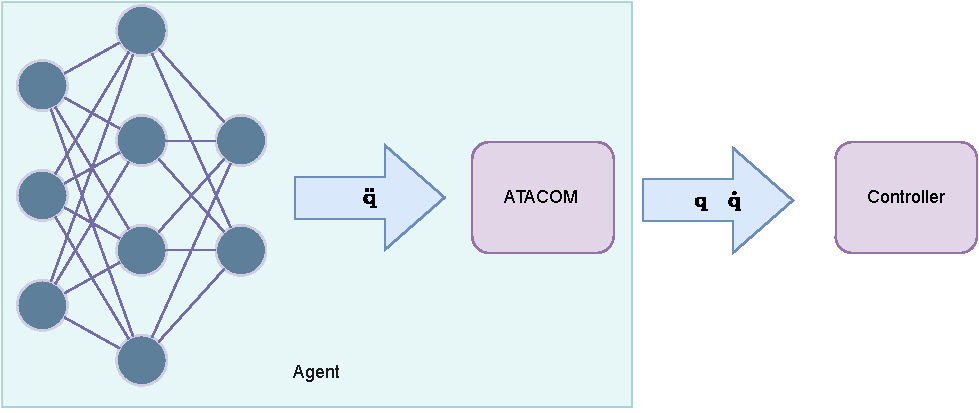
\includegraphics[width=0.8\textwidth]{Images/nn_atacom.pdf}
    \caption{SAC Agent with ATACOM.}
    \label{fig:sac_agent}
\end{figure}

The SAC Agent was used for the \textit{defend}, \textit{counter-attack} and \textit{home} tasks defined in section \label{subsec:reward} with their reward functions.

\subsubsection{Defend and Counter-attack tasks}
For the \textit{defend} and \textit{counter-attack} task a curriculum learning (CL) \cite{CL} approach was used to gradually increase the difficulty of the task and facilitate training.
Manual curricula across three levels of complexity, easy, medium and hard, were devised. These levels differ in the initial configuration of the puck, considering its position and velocity.

\begin{enumerate}
    \item \textbf{Easy}: In the easy level, the puck's velocity was constrained along the y-axis and kept the velocity in the x-axis low.
    Additionally, we positioned the puck at the end of the table, allowing the agent more reaction time.
    \item \textbf{Hard}: Both the x-axis and y-axis puck's velocities were increased, and its initial position was set in the middle of the table.
    \item \textbf{Medium}: The medium task served as an intermediary between the hard and easy tasks.
\end{enumerate}

The agent was trained for a total of 8000 epochs, where each epoch consists in 30 episodes of experience. In the first 3000 epochs the agent was trained with the \text{easy level}. Next a
\textit{soft} switch to the \textit{medium} level task for 1000 epochs increasing the proportion of episodes drawn from the \textit{medium} level task. Between epoch 4000 and 6000 the agent is trained
exclusively on the \textit{medium} level task. As before, a \textit{soft} switch to the \textit{hard} task is performed and finally train exclusively on the \textit{hard} level task for the last 1000 epochs.

\subsubsection{Home task}
In this additional task the goal is to train an agent able to return to the home position fro any arbitrary position.
The initial joint positions for the robot were drawn from a previously collected dataset of configurations 
In this  task the observation space was reduced to only include the joint positions and velocities:
\begin{equation*}
    s = \begin{bmatrix} q & \dot{q} \end{bmatrix}
\end{equation*}
The reward function is described in \ref{subseq:reward}.
No curriculum was needed as the \textit{home} task is simple.
